\documentclass[aspectratio=169]{beamer}
\usepackage{../downey_format_slides}



\usefonttheme{serif}
\setbeamercolor{normal text}{fg=black}

% Make all structural text black (titles, sections, etc.)
\setbeamercolor{structure}{fg=black}

% Frame titles (top title)
\setbeamercolor{frametitle}{fg=black}

% Figure caption ("Figure:")
\setbeamercolor{caption name}{fg=black}
\setbeamercolor{caption}{fg=black}

% Section titles in footer/header
\setbeamercolor{section in head/foot}{fg=black}

% Just in case
\setbeamercolor{title}{fg=black}


% --- Theme setup (minimal) ---
\usetheme{default}
\useoutertheme{default}
\useinnertheme{default}

% Remove navigation symbols
\setbeamertemplate{navigation symbols}{}

% Define your red
% \definecolor{myred}{RGB}{225,120,120}
\definecolor{myred}{RGB}{115,0,10}


\usepackage{color} % color added for editing
\newcommand{\bl}[1]{\textcolor[rgb]{0.00,0.00,1.00}{#1}}
\newcommand{\gr}[1]{\textcolor[rgb]{0.00,0.50,0.00}{#1}}
\newcommand{\rd}[1]{\textcolor[rgb]{0.75,0.00,0.00}{#1}}
\newcommand{\tl}[1]{\textcolor[rgb]{0,0.6,0.60}{#1}}

\usepackage{booktabs}
\usepackage{bm}
\usepackage{mdframed}
\usepackage{xcolor}

% --- Custom footline ---
\setbeamertemplate{footline}{
\leavevmode

% Thin red line (moved to TOP)
\begin{beamercolorbox}[wd=\paperwidth,ht=0.1ex]{}
\color{myred}\rule{\paperwidth}{0.1ex}
\end{beamercolorbox}

\hbox{
\begin{beamercolorbox}[wd=\paperwidth,ht=2.5ex,dp=1ex]{}
\hspace{1em}
\insertsection
\hfill
\insertframenumber{} / \inserttotalframenumber
\hspace{1em}
\end{beamercolorbox}
}
}

% Remove headline entirely
\setbeamertemplate{headline}{}

% Optional: clean fonts
\setbeamerfont{footline}{size=\small}







\title{Chapter~6~Decision Trees}
\author{Austin R.J. Downey}
\date{}

\begin{document}

\section{Machine Learning for Engineering Problem Solving}
\frame{\titlepage}


\section{Chapter~6~Decision Trees}

\section{6.1~Decision Tree Classification}



\begin{frame}{Decision Trees}
	\begin{columns}
		
		\column{0.42\textwidth}
		
		Decision Trees are flexible models used for:
		
		\begin{itemize}
			\item Classification
			\item Regression
			\item Multi-output prediction
		\end{itemize}
		
		\vspace{0.5em}
		
		Key ideas:
		\begin{itemize}
			\item Split data using simple rules
			\item Build a tree of decisions
			\item Make predictions by following a path
		\end{itemize}
		
		\vspace{0.5em}
		
		They are also the building blocks of Random Forests.
		
		\column{0.58\textwidth}
		\centering
		
\includegraphics[
		width=0.75\textwidth,
		trim={3.3in 0.15in 0in 0in},
		clip
		]{../figures/decision_tree_basic_concept}
		
		\vspace{0.3em}
		{\small Basic concept of a decision tree.}
		
	\end{columns}
\end{frame}

%------------------------------------------------

\begin{frame}{Decision Trees}
	\begin{columns}
		
		\column{0.42\textwidth}
		
		Decision Trees are flexible models used for:
		
		\begin{itemize}
			\item Classification
			\item Regression
			\item Multi-output prediction
		\end{itemize}
		
		\vspace{0.5em}
		
		Key ideas:
		\begin{itemize}
			\item Split data using simple rules
			\item Build a tree of decisions
			\item Make predictions by following a path
		\end{itemize}
		
		\vspace{0.5em}
		
		They are also the building blocks of Random Forests.
		
		\column{0.58\textwidth}
		\centering
		
		
\includegraphics[
		width=0.6\textwidth,
		trim={0in 0in 3.0in 0in},
		clip
		]{../figures/decision_tree_basic_concept}
		
		\vspace{0.4em}
		
		
\includegraphics[
		width=0.6\textwidth,
		trim={3.3in 0in 0in 0in},
		clip
		]{../figures/decision_tree_basic_concept}
		
		\vspace{0.3em}
		{\small Basic concept of a decision tree.}
		
	\end{columns}
\end{frame}

%------------------------------------------------

\begin{frame}{Decision Tree Classification}
	\begin{columns}
		
		\column{0.42\textwidth}
		
		A decision tree partitions the feature space into regions.
		
		\vspace{0.5em}
		
		For the Iris dataset:
		
		\begin{itemize}
			\item Root split:
			\[
			\text{petal length} \le 2.45
			\]
			\item Second split:
			\[
			\text{petal width} \le 1.75
			\]
		\end{itemize}
		
		\vspace{0.5em}
		
		Each region is assigned a predicted class.
		
		\column{0.58\textwidth}
		\centering
		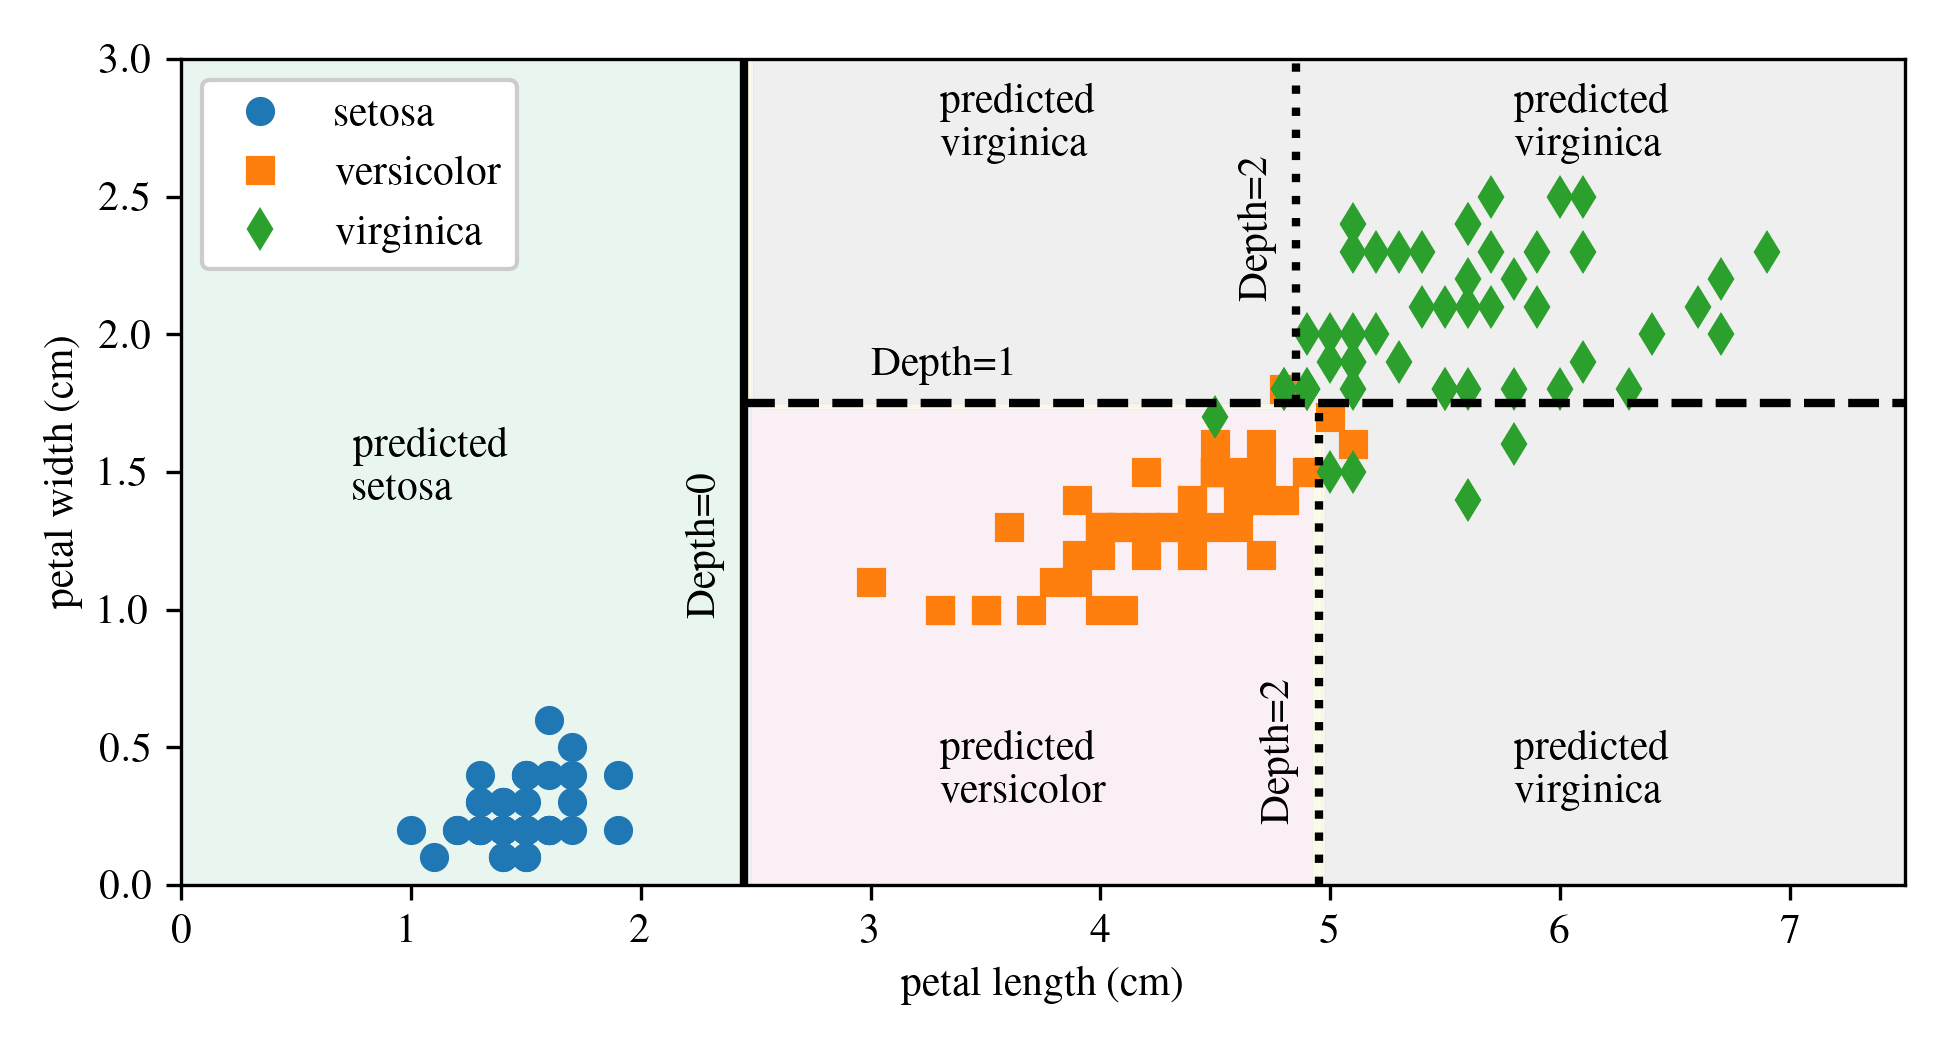
\includegraphics[width=\textwidth]{../figures/decision_tree_boundaries}
		
		\vspace{0.3em}
		{\small Decision tree decision boundaries.}
		
	\end{columns}
\end{frame}

%------------------------------------------------

\begin{frame}{Reading a Decision Tree}
	\begin{columns}
		
		\column{0.38\textwidth}
		
		To classify a new sample:
		
		\begin{enumerate}
			\item Start at the root node
			\item Answer the split question
			\item Move left or right
			\item Continue until a leaf node is reached
		\end{enumerate}
		
		\vspace{0.5em}
		
		The leaf node gives the predicted class.
		
		\column{0.62\textwidth}
		\centering
		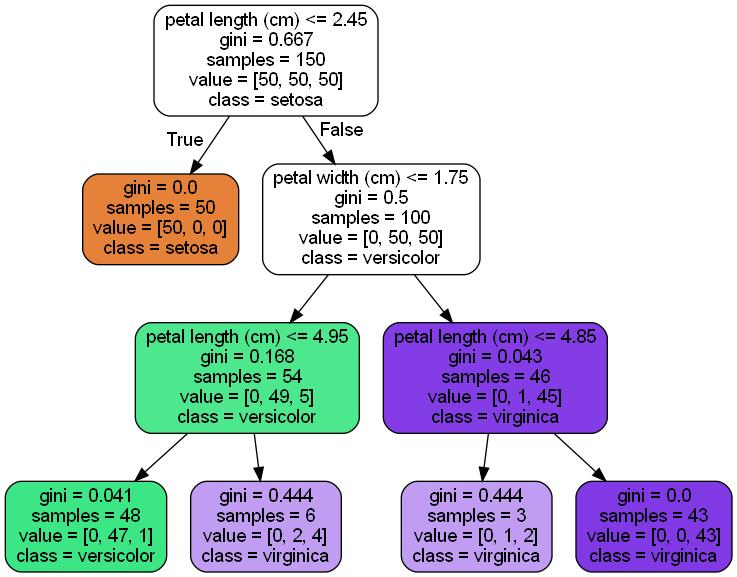
\includegraphics[height=0.72\textheight]{../figures/Iris_decision_tree}
		
		\vspace{0.3em}
		{\small Decision tree trained on the Iris dataset.}
		
	\end{columns}
\end{frame}

% ------------------------------------------------

\begin{frame}{Node Information}
	
	Each node in a classification tree stores useful information.
	
	\vspace{0.5em}
	
	\begin{itemize}
		\item \textbf{class}: predicted class at the node
		\item \textbf{samples}: number of training instances that reach the node
		\item \textbf{value}: class counts at the node
		\item \textbf{gini}: impurity of the node
	\end{itemize}
	
	\vspace{0.75em}
	
	A node is pure when all samples belong to the same class:
	
	\[
	G_i = 0
	\]
	
	\vspace{0.5em}
	
	Darker node colors indicate purer predictions.
	
\end{frame}

% ------------------------------------------------

\begin{frame}{Gini Impurity}
	
	Gini impurity measures how mixed the classes are at a node.
	
	\[
	G_i
	=
	1 -
	\sum_{k=1}^{n}p_{i,k}^{2}
	\]
	
	\vspace{0.5em}
	
	where:
	
	\begin{itemize}
		\item $p_{i,k}$ is the proportion of class $k$ at node $i$
		\item $G_i=0$ means the node is pure
		\item Larger values indicate more mixed classes
	\end{itemize}
	
	\vspace{0.75em}
	
	Example:
	\[
	1-\left(\frac{0}{54}\right)^2
	-\left(\frac{49}{54}\right)^2
	-\left(\frac{5}{54}\right)^2
	\approx 0.168
	\]
	
\end{frame}

% ------------------------------------------------

\begin{frame}{Class Probability Estimation}
	
	Decision Trees can estimate class probabilities.
	
	\vspace{0.5em}
	
	Procedure:
	
	\begin{enumerate}
		\item Follow the sample to a leaf node
		\item Count the training samples in that leaf
		\item Compute the fraction belonging to each class
	\end{enumerate}
	
	\vspace{0.75em}
	
	Example leaf node:
	
	\[
	\text{value} = [0,\;49,\;5]
	\]
	
	\vspace{0.5em}
	
	Probabilities:
	
	\[
	P(\text{setosa}) = 0\% \text{,  } P(\text{versicolor}) = \frac{49}{54}=90.7\%  \text{, and } P(\text{virginica}) = \frac{5}{54}=9.3\%
	\]
	
\end{frame}

% ------------------------------------------------

\begin{frame}{Example 6.1: Decision Tree Classifier}
	
	\begin{itemize}
		\item Use \texttt{DecisionTreeClassifier}
		\item Classify Iris species using petal features
		\item Train a tree with a limited depth
		\item Visualize the learned decision rules with Graphviz
	\end{itemize}
	
	\vspace{0.5em}
	
	The exported tree shows:
	
	\begin{itemize}
		\item Feature thresholds
		\item Gini impurity
		\item Sample counts
		\item Class distributions
	\end{itemize}
	
	\vspace{0.5em}
	
	Graphviz viewer:
	
	\vspace{0.3em}
	
	\url{https://dreampuf.github.io/GraphvizOnline/}
	
\end{frame}

% ------------------------------------------------

\section{6.2~The CART Training Algorithm}

\begin{frame}{The CART Training Algorithm}
	\begin{columns}
		
		\column{0.44\textwidth}
		
		Scikit-Learn trains decision trees using CART:
		
		\[
		\text{Classification and Regression Trees}
		\]
		
		\vspace{0.5em}
		
		At each node, CART chooses:
		
		\begin{itemize}
			\item A feature $k$
			\item A threshold $t_k$
		\end{itemize}
		
		\vspace{0.5em}
		
		The goal is to create child nodes that are as pure as possible.
		
		\column{0.56\textwidth}
		\centering
		
\includegraphics[width=\textwidth]{../figures/CART_algorithm}
		
		\vspace{0.3em}
		{\small CART recursively grows the tree.}
		
	\end{columns}
\end{frame}

%------------------------------------------------

\begin{frame}{CART Objective}
	
	At each split, CART minimizes:
	
	\[
	J(k,t_k)
	=
	\frac{m_{\text{left}}}{m}G_{\text{left}}
	+
	\frac{m_{\text{right}}}{m}G_{\text{right}}
	\]
	
	\vspace{0.5em}
	
	where:
	
	\begin{itemize}
		\item $G_{\text{left}}$ and $G_{\text{right}}$ are impurity values
		\item $m_{\text{left}}$ and $m_{\text{right}}$ are sample counts
		\item $m$ is the total number of samples at the current node
	\end{itemize}
	
	\vspace{0.5em}
	
	The tree grows recursively until:
	
	\begin{itemize}
		\item A maximum depth is reached
		\item No useful impurity-reducing split remains
	\end{itemize}
	
\end{frame}

%------------------------------------------------

\begin{frame}{Regularizing Decision Trees}
	
	Decision Trees can easily overfit when they are allowed to grow too freely.
	
	\vspace{0.5em}
	
	Regularization works by limiting the complexity of the tree.
	
	\vspace{0.5em}
	
	Important Scikit-Learn hyperparameters:
	
	\begin{itemize}
		\item \texttt{max\_depth}: limits how deep the tree can grow
		\item \texttt{min\_samples\_split}: requires enough samples before splitting
		\item \texttt{min\_samples\_leaf}: requires enough samples in each leaf
		\item \texttt{max\_leaf\_nodes}: limits the number of leaf nodes
		\item \texttt{max\_features}: limits features considered at each split
	\end{itemize}
	
	\vspace{0.5em}
	
	General rule:
	
	\begin{itemize}
		\item Increase \texttt{min\_[...]} values to require more data before splitting
		\item Decrease \texttt{max\_[...]} values to cap tree size and complexity
	\end{itemize}
	
\end{frame}

%------------------------------------------------

\begin{frame}{Regularization Effects}
	\begin{columns}
		
		\column{0.42\textwidth}
		
		An unrestricted tree may fit noise in the training data.
		
		\vspace{0.5em}
		
		Adding restrictions can improve generalization.
		
		\vspace{0.5em}
		
		Example:
		
		\[
		\texttt{min\_samples\_leaf}=4
		\]
		
		\vspace{0.5em}
		
		This prevents leaves from being created from very small groups of samples.
		
		\column{0.58\textwidth}
		\centering
		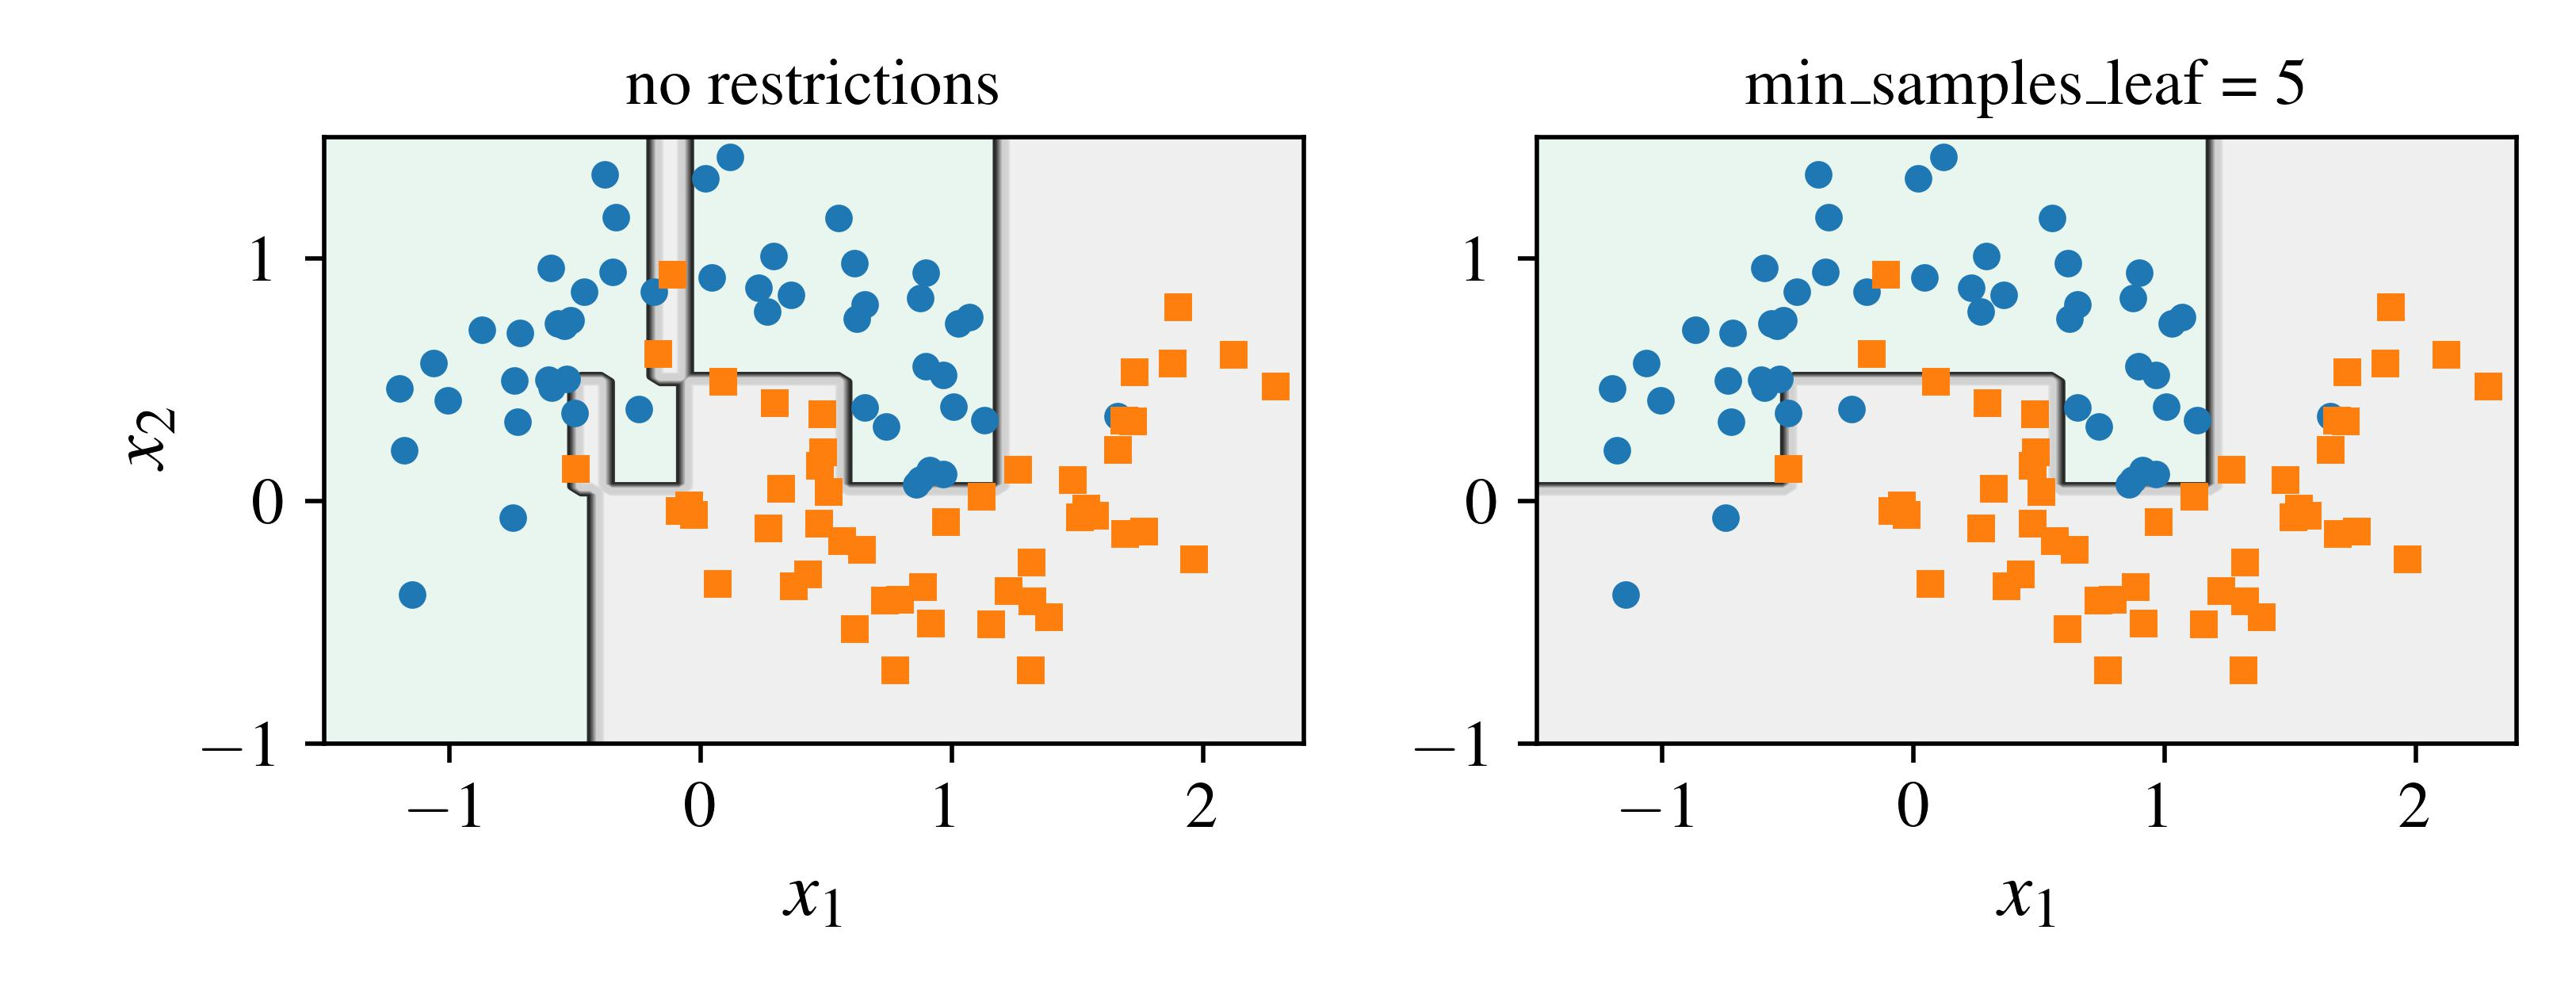
\includegraphics[width=\textwidth]{../figures/decision_tree_regularization}
		
		\vspace{0.3em}
		{\small Regularization using \texttt{min\_samples\_leaf}.}
		
	\end{columns}
\end{frame}

%------------------------------------------------

\begin{frame}{Computational Complexity}
	
	Prediction is fast.
	
	\vspace{0.5em}
	
	A prediction follows one path from the root to a leaf:
	
	\[
	T_{\text{predict}}
	=
	O(\log_2 m)
	\]
	
	\vspace{0.5em}
	
	Training is more expensive:
	
	\[
	T_{\text{train}}
	=
	O(nm\log m)
	\]
	
	\vspace{0.5em}
	
	where:
	
	\begin{itemize}
		\item $m$: number of training instances
		\item $n$: number of input features
	\end{itemize}
	
	\vspace{0.5em}
	
	Decision Trees are especially efficient at prediction time.
	
\end{frame}

%------------------------------------------------

\begin{frame}{Gini Impurity vs. Entropy}
	
	Scikit-Learn uses Gini impurity by default.
	
	\vspace{0.5em}
	
	Entropy is another impurity measure:
	
	\[
	H_i
	=
	-
	\sum_{k=1}^{n}
	p_{i,k}\log_2(p_{i,k})
	\]
	
	\vspace{0.5em}
	
	Comparison:
	
	\begin{itemize}
		\item Gini is slightly faster to compute
		\item Gini often isolates the most frequent class
		\item Entropy tends to produce more balanced trees
	\end{itemize}
	
	\vspace{0.5em}
	
	In practice, both usually produce similar trees.
	
\end{frame}

%------------------------------------------------

\section{6.3~Decision Tree Regression}

\begin{frame}{Decision Tree Regression}
	\begin{columns}
		
		\column{0.42\textwidth}
		
		Decision Trees can also perform regression.
		
		\vspace{0.5em}
		
		Instead of predicting a class, each leaf predicts:
		
		\[
		\hat{y}_{\text{node}}
		\]
		
		\vspace{0.5em}
		
		This value is the average target value of the training instances in that leaf.
		
		\vspace{0.5em}
		
		The model creates piecewise-constant predictions.
		
		\column{0.58\textwidth}
		\centering
		
		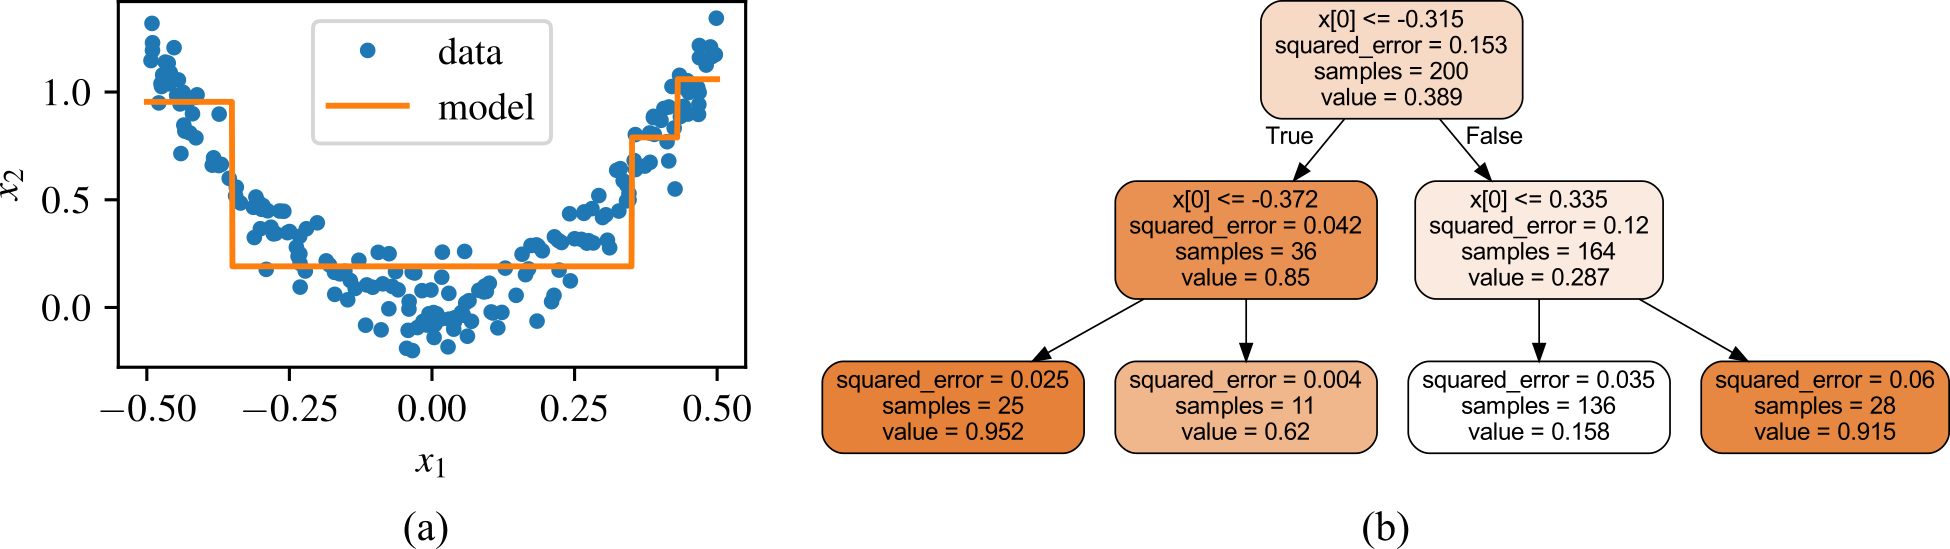
\includegraphics[
			width=0.6\textwidth,
			trim={0in 0.2in 3.8in 0in},
			clip
		]{../figures/decision_tree_regression}
		
		\vspace{0.4em}
		
		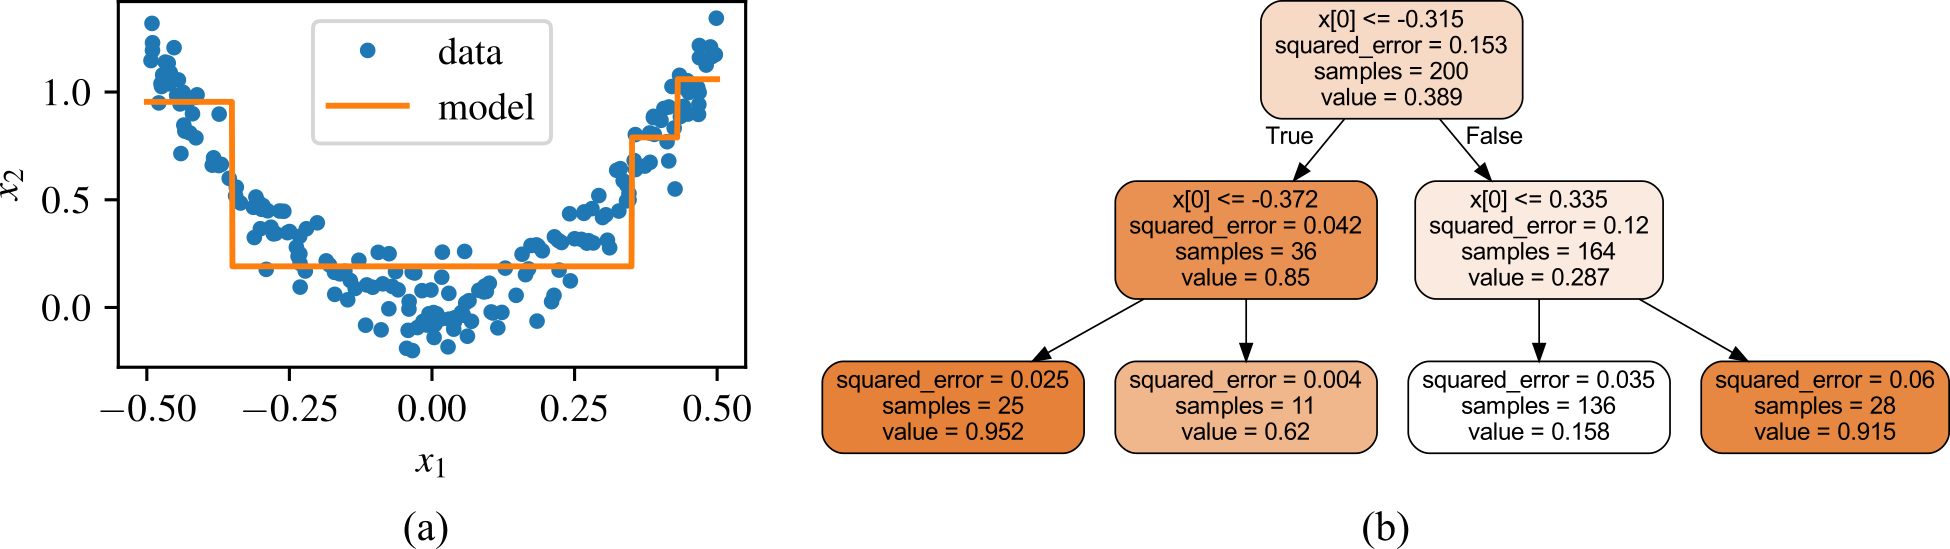
\includegraphics[
			width=0.6\textwidth,
			trim={2.7in 0.2in 0in 0in},
			clip
		]{../figures/decision_tree_regression}
		
		\vspace{0.3em}
		{\small Decision Tree regression model and tree.}
		
	\end{columns}
\end{frame}

%------------------------------------------------

\begin{frame}{Tree Depth in Regression}
	\begin{columns}
		
		\column{0.42\textwidth}
		
		Increasing tree depth creates more prediction regions.
		
		\vspace{0.5em}
		
		Shallow tree:
		
		\begin{itemize}
			\item Fewer regions
			\item Simpler model
			\item More bias
		\end{itemize}
		
		\vspace{0.5em}
		
		Deeper tree:
		
		\begin{itemize}
			\item More regions
			\item More flexible model
			\item Higher risk of overfitting
		\end{itemize}
		
		\column{0.58\textwidth}
		\centering
		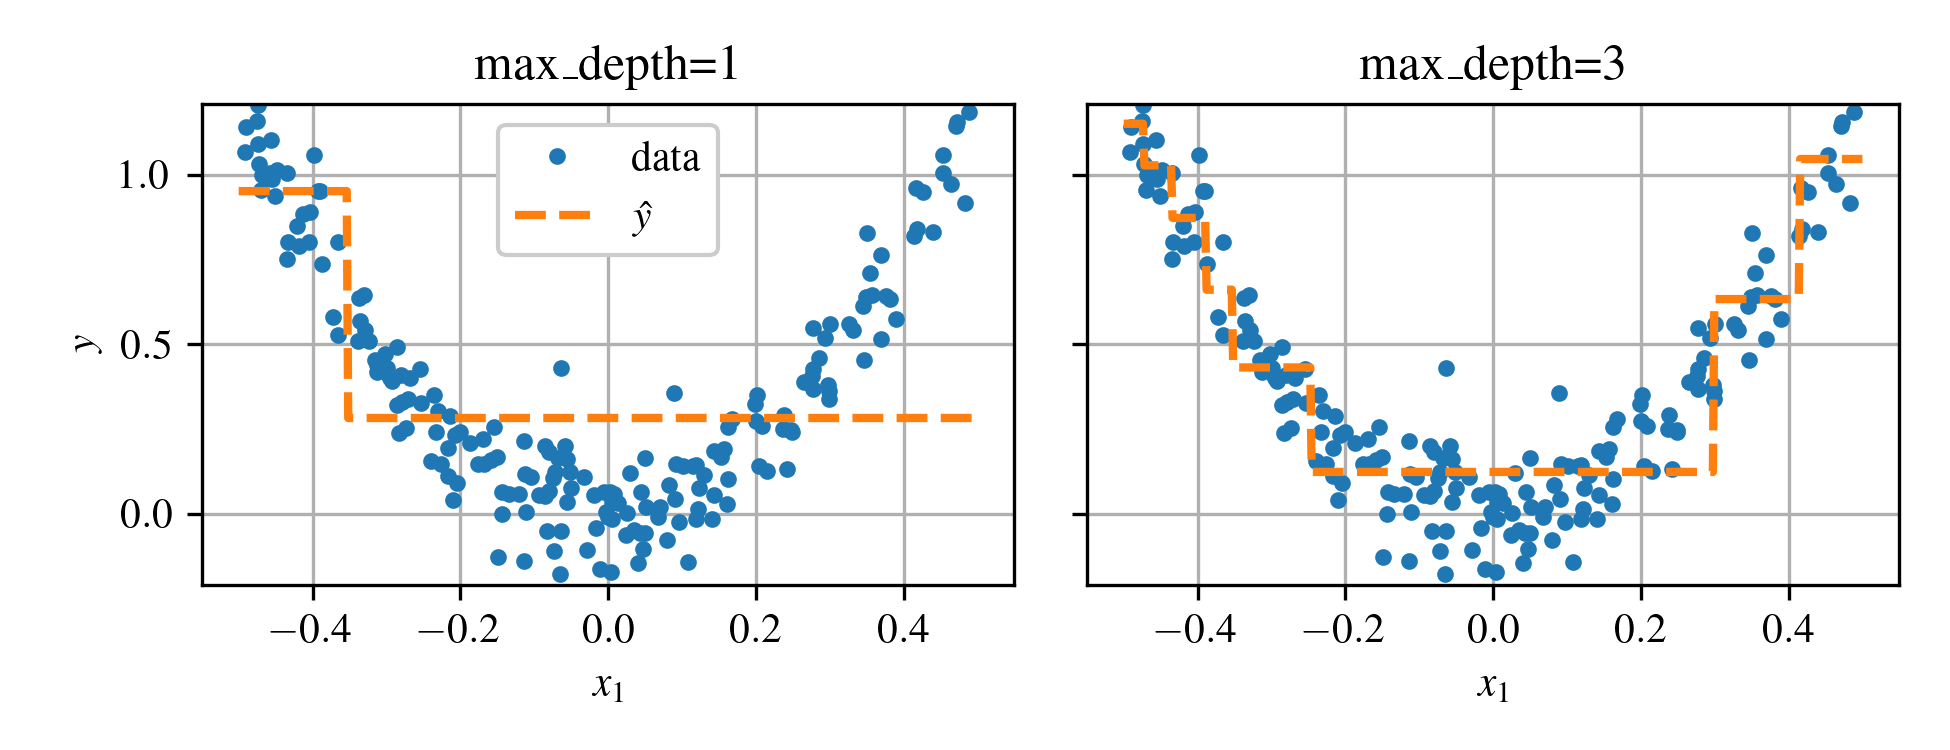
\includegraphics[width=\textwidth]{../figures/decision_tree_regression_prediction}
		
		\vspace{0.3em}
		{\small Regression trees with different depths.}
		
	\end{columns}
\end{frame}

%------------------------------------------------

\begin{frame}{Regression Tree Cost Function}
	
	For regression, CART minimizes MSE instead of impurity.
	
	\[
	J(k,t_k)
	=
	\frac{m_{\text{left}}}{m}
	\text{MSE}_{\text{left}}
	+
	\frac{m_{\text{right}}}{m}
	\text{MSE}_{\text{right}}
	\]
	
	\vspace{0.5em}
	
	At each node:
	
	\[
	\text{MSE}_{\text{node}}
	=
	\sum_{i\in\text{node}}
	\left(\hat{y}_{\text{node}} - y^{(i)}\right)^2
	\]
	
	\[
	\hat{y}_{\text{node}}
	=
	\frac{1}{m_{\text{node}}}
	\sum_{i\in\text{node}}y^{(i)}
	\]
	
	\vspace{0.5em}
	
	The tree chooses splits that reduce prediction error.
	
\end{frame}

%------------------------------------------------

\begin{frame}{Regularizing Regression Trees}
	\begin{columns}
		
		\column{0.42\textwidth}
		
		Regression trees can also overfit.
		
		\vspace{0.5em}
		
		Without regularization:
		
		\begin{itemize}
			\item Tree follows noise
			\item Predictions become jagged
		\end{itemize}
		
		\vspace{0.5em}
		
		With regularization:
		
		\begin{itemize}
			\item Leaves contain more samples
			\item Predictions are smoother
			\item Generalization improves
		\end{itemize}
		
		\column{0.58\textwidth}
		\centering
		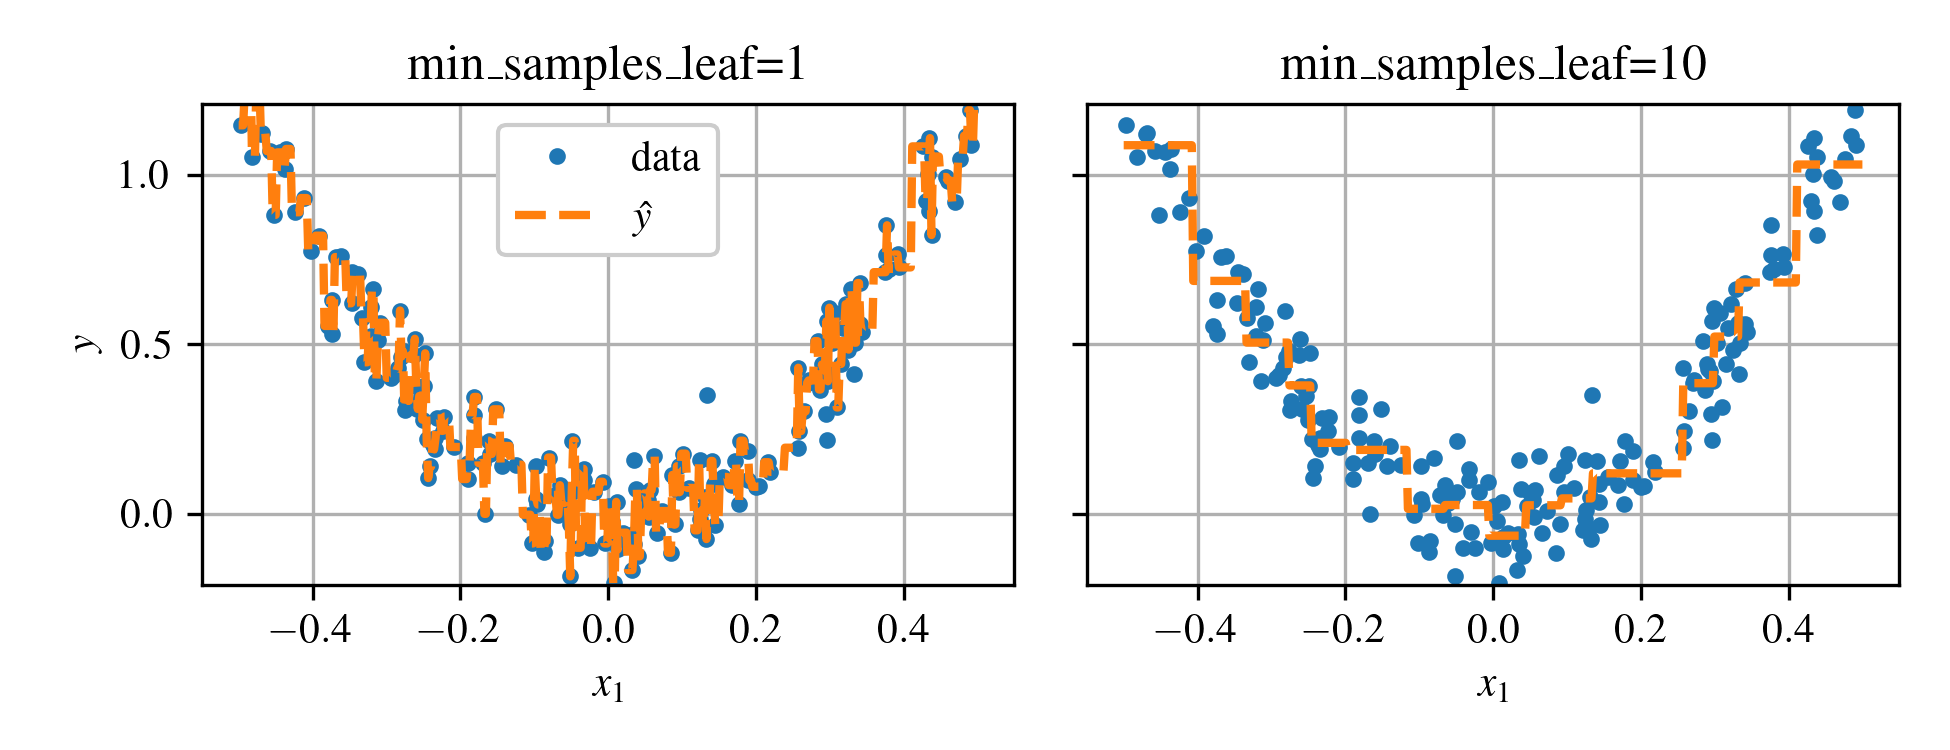
\includegraphics[width=\textwidth]{../figures/decision_tree_regression_regularized}
		
		\vspace{0.3em}
		{\small Effect of \texttt{min\_samples\_leaf} on regression trees.}
		
	\end{columns}
\end{frame}

% ------------------------------------------------

\begin{frame}{Example 6.2: Decision Tree Regression}
	
	\begin{itemize}
		\item Use \texttt{DecisionTreeRegressor}
		\item Fit a nonlinear relationship between input and output data
		\item Train a tree with limited depth
		\item Visualize the regression tree using Graphviz
	\end{itemize}
	
	\vspace{0.5em}
	
	This example shows how a tree partitions the input space into regions.
	
	\vspace{0.5em}
	
	Each region predicts the average target value of the samples it contains.
	
\end{frame}

% -------------------------------------------------

\section{6.4~Random Forest}

\begin{frame}{Instability: Feature Orientation}
	\begin{columns}
		
		\column{0.42\textwidth}
		
		Decision Trees prefer orthogonal splits.
		
		\vspace{0.5em}
		
		This makes them sensitive to feature orientation.
		
		\vspace{0.5em}
		
		A simple rotation of the data can produce:
		
		\begin{itemize}
			\item More complex boundaries
			\item Poorer generalization
			\item Less stable predictions
		\end{itemize}
		
		\vspace{0.5em}
		
		PCA can sometimes help reorient the data.
		
		\column{0.58\textwidth}
		\centering
		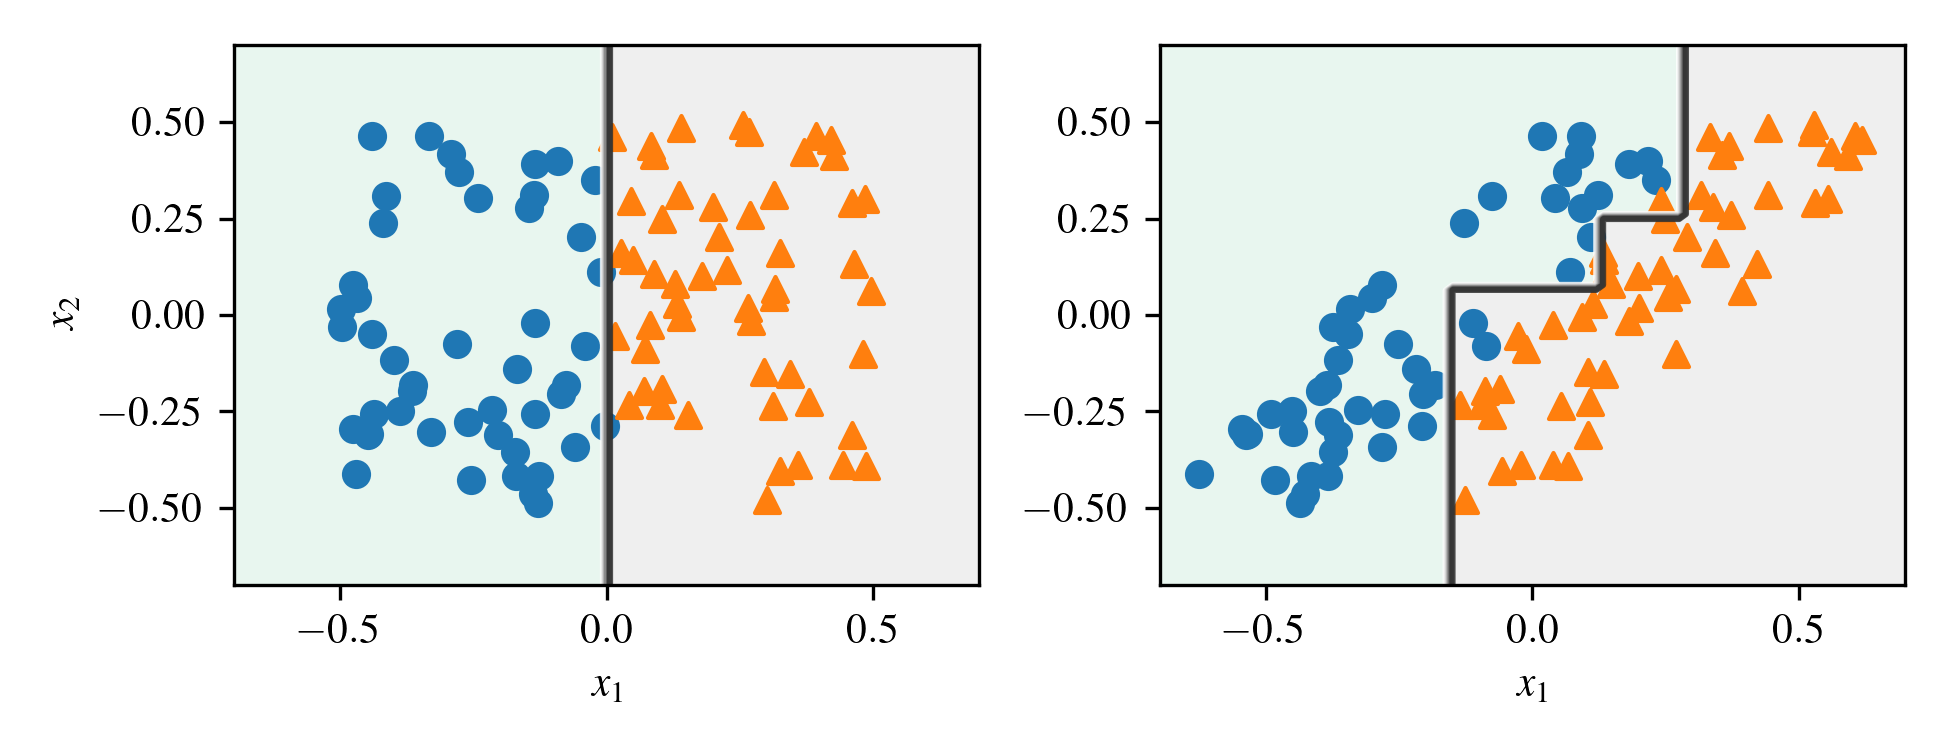
\includegraphics[width=\textwidth]{../figures/decision_tree_training_rotation}
		
		\vspace{0.3em}
		{\small Sensitivity to feature rotation.}
		
	\end{columns}
\end{frame}

% -------------------------------------------------



\begin{frame}{Instability: Training Variation}
	\begin{columns}
		
		\column{0.42\textwidth}
		
		Decision Trees can change significantly with small training variations.
		
		\vspace{0.5em}
		
		Sources of variation:
		
		\begin{itemize}
			\item Random number seed
			\item Equal-quality candidate splits
			\item Small changes in training data
		\end{itemize}
		
		\vspace{0.5em}
		
		To improve reproducibility:
		
		\[
		\texttt{random\_state}
		\]
		
		\vspace{0.5em}
		
		can be fixed during training.
		
		\column{0.58\textwidth}
		\centering
		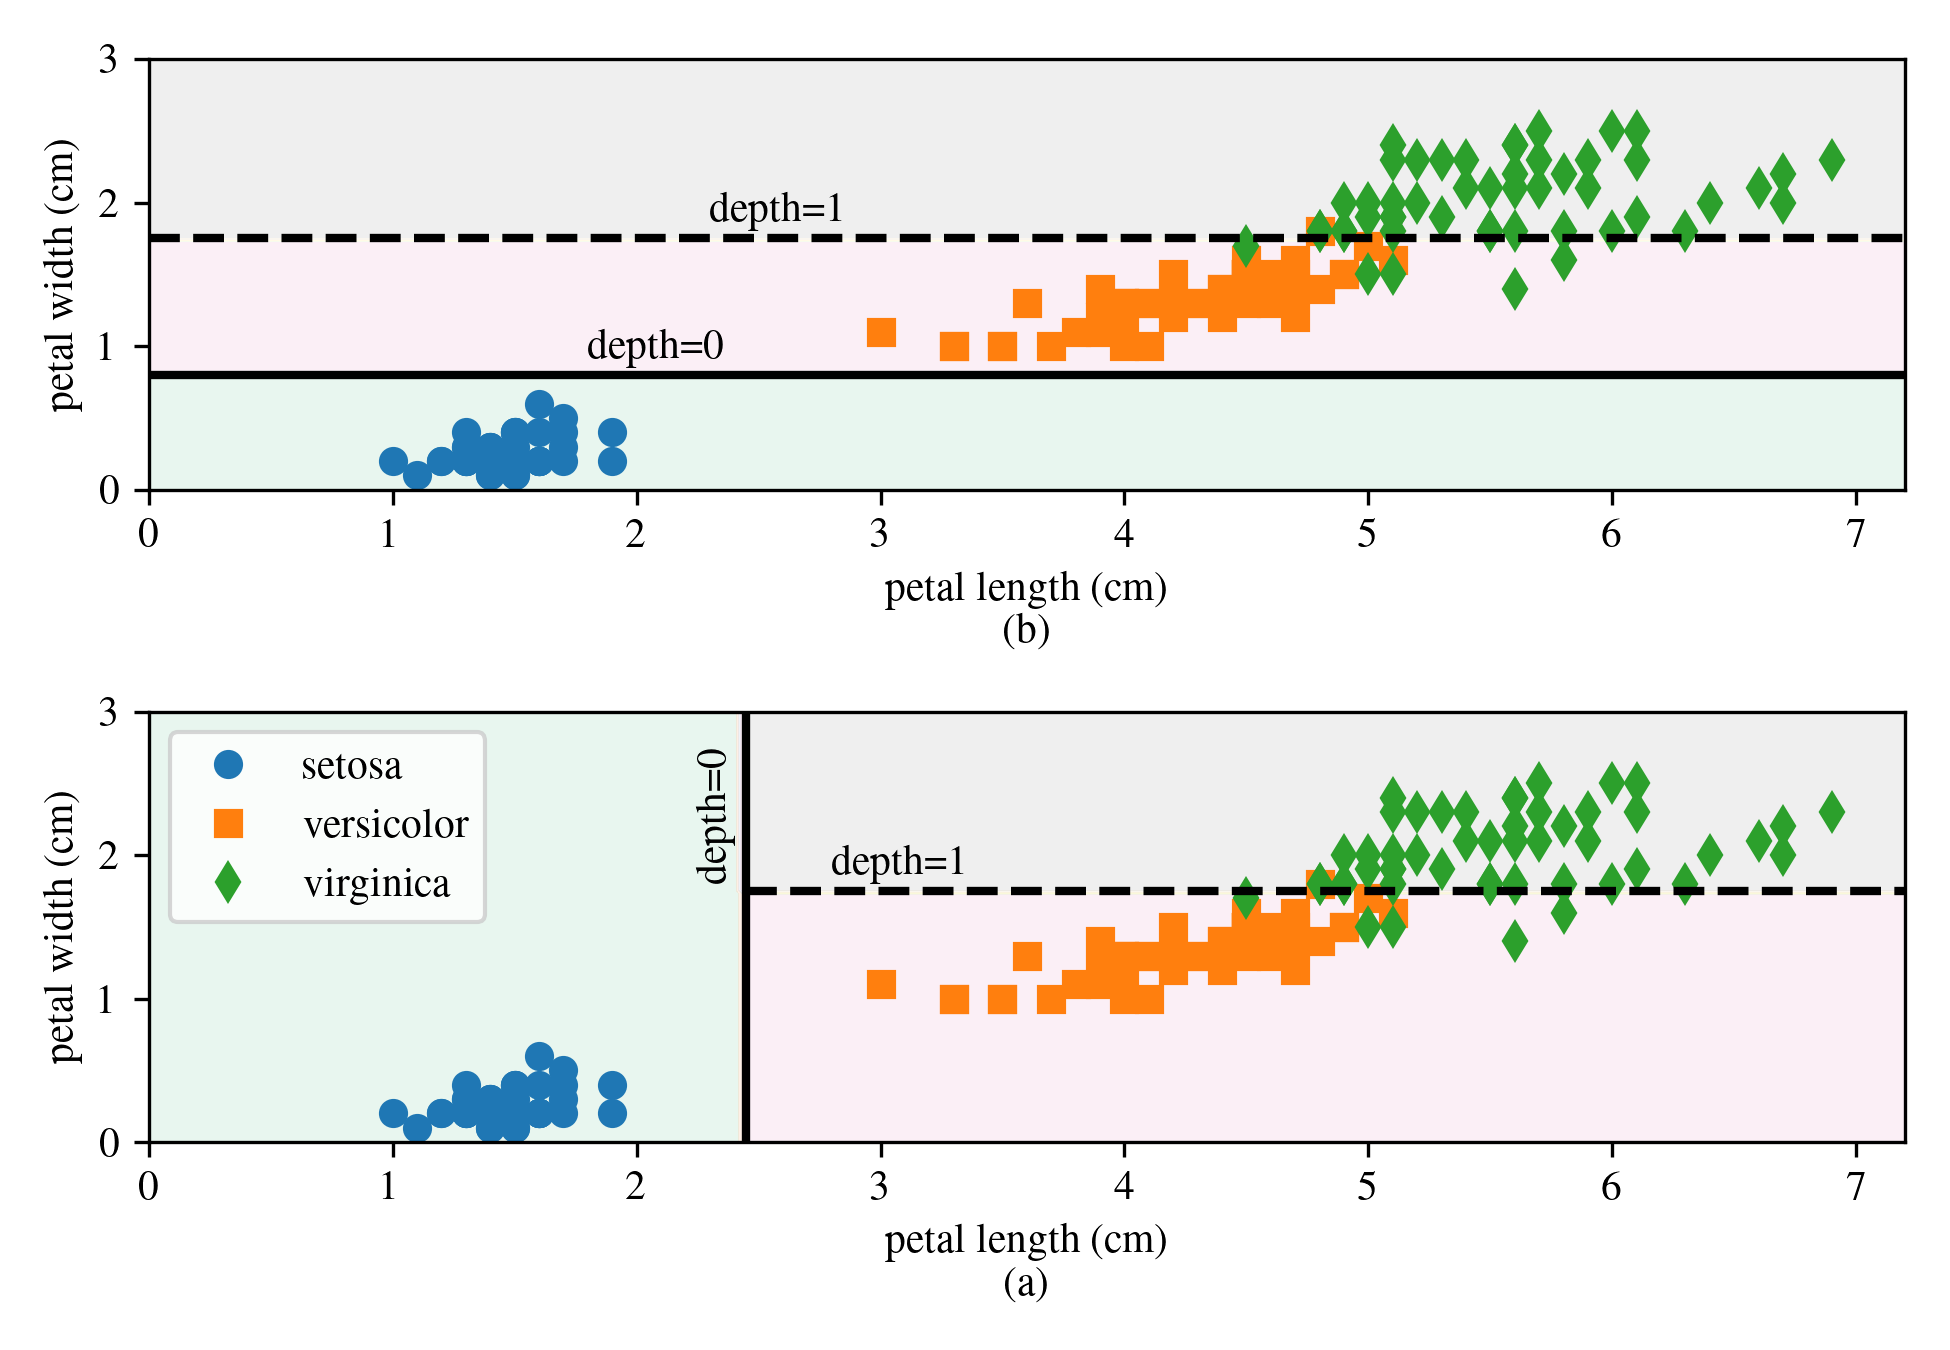
\includegraphics[width=\textwidth]{../figures/decision_tree_sensitivity}
		
		\vspace{0.3em}
		{\small Sensitivity to initial conditions.}
		
	\end{columns}
\end{frame}

% -------------------------------------------------



\begin{frame}{Random Forests}
	\begin{columns}
		
		\column{0.42\textwidth}
		
		A Random Forest builds many Decision Trees.
		
		\vspace{0.5em}
		
		Each tree is trained using:
		
		\begin{itemize}
			\item A bootstrap sample of the data
			\item A random subset of features
		\end{itemize}
		
		\vspace{0.5em}
		
		Predictions are combined by:
		
		\begin{itemize}
			\item Majority vote for classification
			\item Averaging for regression
		\end{itemize}
		
		\vspace{0.5em}
		
		This reduces variance compared with a single tree.
		
		\column{0.58\textwidth}
		\centering
		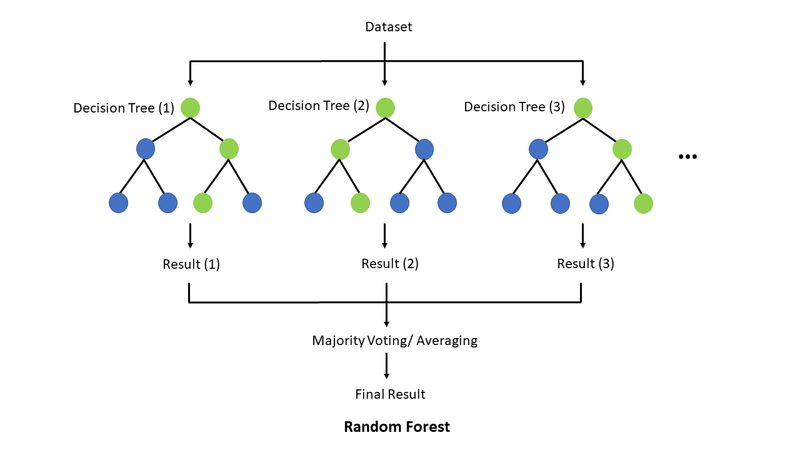
\includegraphics[width=\textwidth]{../figures/random_forest}
		
		\vspace{0.3em}
		{\small Random forest with majority voting.}
		
	\end{columns}
\end{frame}

















\end{document}




